\documentclass[twocolumn, 10pt]{article}

\usepackage{amsmath}
\usepackage{graphicx}
\usepackage{float}
\usepackage{listings}
\graphicspath{ {./images/} }

\title{2XC3 - Lab 1 Report}
\author{Oleg Glotov\\ L03, 400174037\\ glotovo@mcmaster.ca \and Emma Willson\\ L02, 400309856\\ willsone@mcmaster.ca}


\begin{document}
\maketitle
\section{Git Setup}\label{sec:git}
The group began by setting up out github accounts and the repository. The visibility was set to private to comply with McMaster's code of conduct.

\begin{figure}[H]
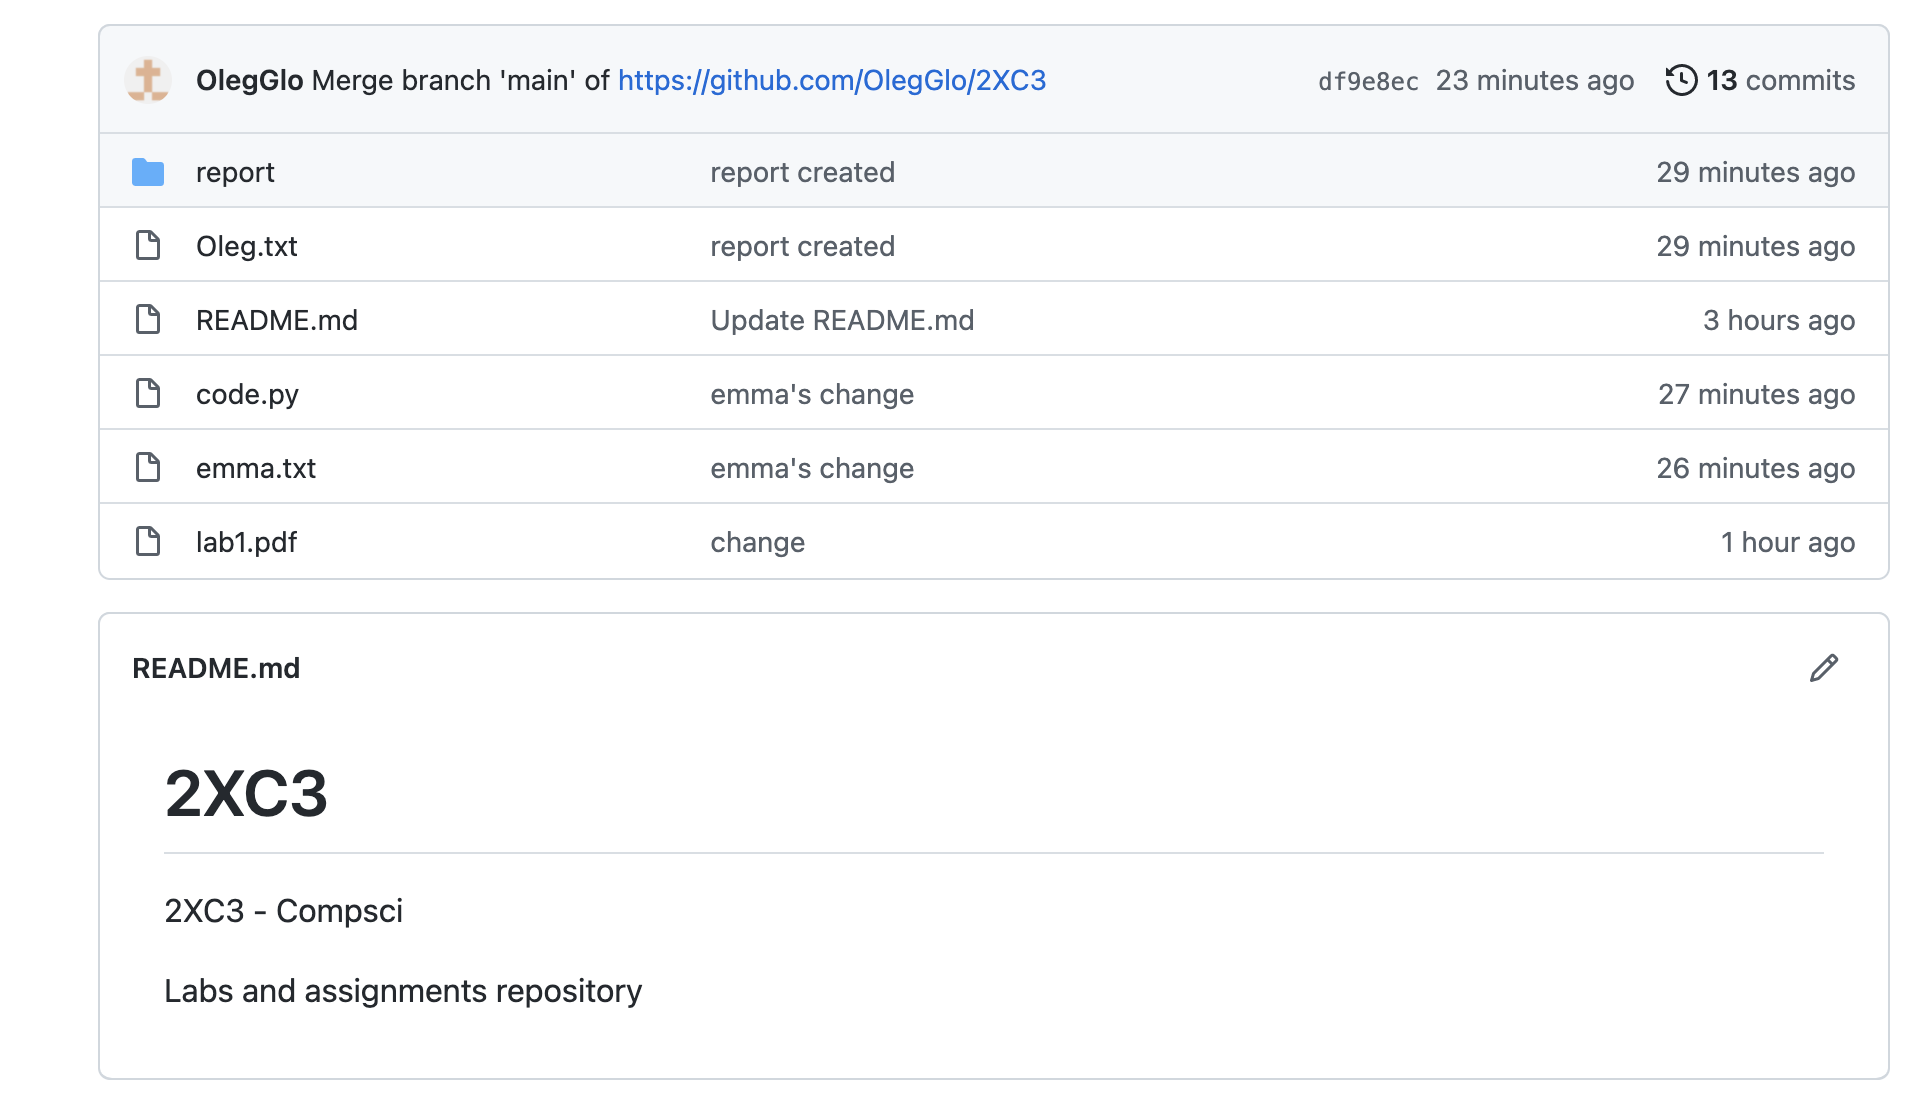
\includegraphics[width=\linewidth]{img1}
\end{figure}

Both of us has access to the repository. We choose to work with github directly thorough our VSCode IDE since it fully integrates git commands and simplifies the workflow.

\section{Git commands}

We experimented with several git commands, including merge, reset and revert, which are shown below. 

First, we experimented with merge by editing the same line in a text file and then pushing that change to the repository. In VS Code, we were shown the conflict and given the option to choose a version of the file, to merge the two, or reject both changes.

\begin{figure}[H]
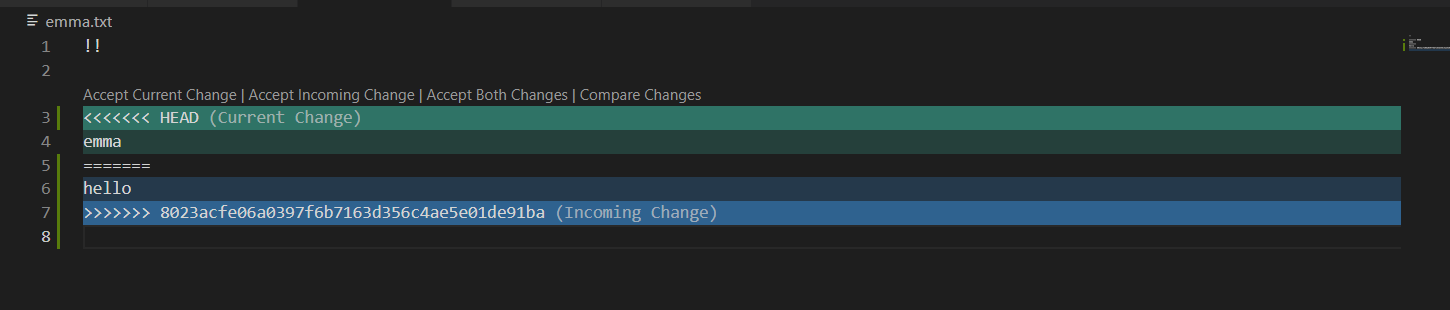
\includegraphics[width=\linewidth]{merge}
\end{figure}

Then, we used reset to undo some changes made to this report file. Since reset moves the branch that HEAD points to, to a different commit, it's easy to undo uncommitted changes to the file. A downside to reset is that the undone changes are lost.

\begin{figure}[H]
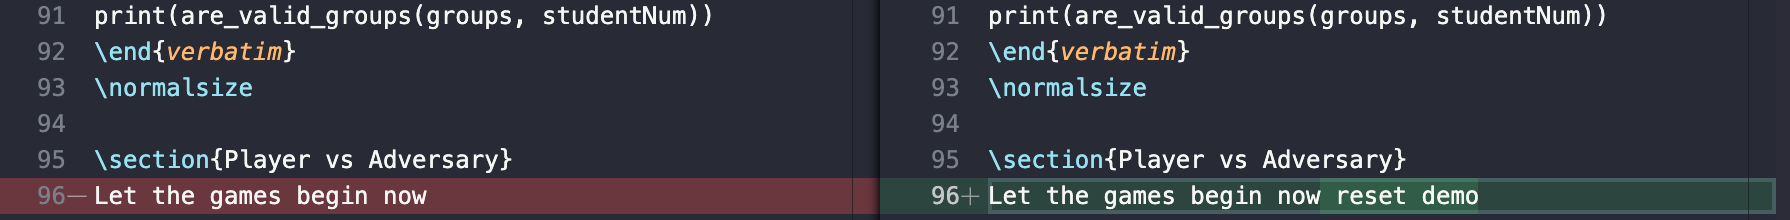
\includegraphics[width=\linewidth]{reset}
\end{figure}

Finally, we used revert to undo some changes made to another file. Revert creates a new commit that reverses the changes made by the previous commit. This provides clear documentation of previous versions and allows us to easily return to those before the reverted one.

\begin{figure}[H]
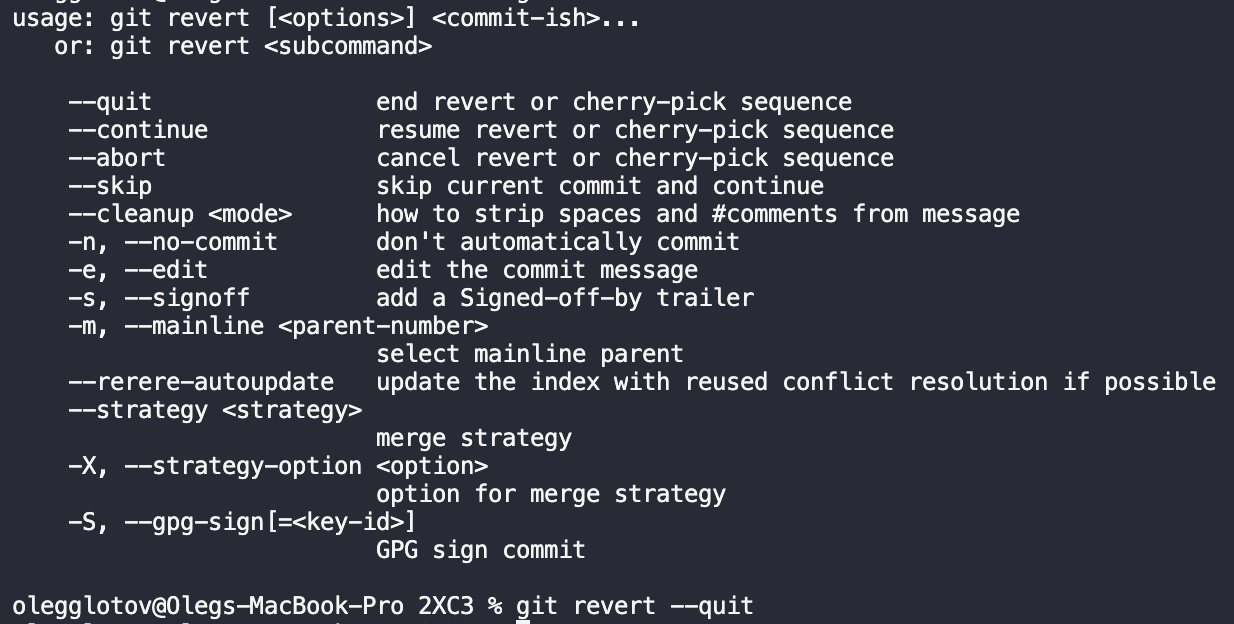
\includegraphics[width=\linewidth]{revert}
\end{figure}

\section{Code.py}

Both group member's code is provided below. After consulting we decided to combine both of ours solution into the final product in the file code.py not provided here.

\paragraph{Oleg's version:}

\footnotesize
\begin{verbatim}
def are_valid_groups(groups, studentNum):

    length = len(studentNum)
    count = 0
    
    for group in groups:
        count = 0
        for students in studentNum:
            if (group.count(students) == 0):
                break
            if (group.count(students) == 1):
                count += 1
        
        if count == length:
            return True
        
    return False
\end{verbatim}
\normalsize

\paragraph{Emma's version:}

\footnotesize
\begin{verbatim}
def are_valid_groups(nums, groups):
    valid = True
    for num in nums:
        valid = False
        for group in groups:
            if (num in group): 
                valid = True
                break
        if (not valid):
            return False
    return True
\end{verbatim}
\normalsize

\section{Player vs Adversary}

The code for the string conversion initially would look like this:

\footnotesize
\begin{verbatim}
def are_valid_groups(groups, studentNum):

length = len(studentNum)
countID = 0   
for students in studentNum:
    count = 0
    for group in groups:
        if (group.count(students) > 0):
            count += group.count(students)

    if (count == 1):
        countID += 1
    else:
        return False
if (countID == length):
    return True
return False
\end{verbatim}
\normalsize

The process of solving merge conflicts would remain consistent throughout the lab and is very similar to how it was described earlier.

The player would simply have to decline or accept the changes made by the adversary when pushing their changes. In the case of confusion the \textbf{git reset} command can be used.

When a merge conflict arises, the choice between accepting the changes, keeping the current code or accept both can be made. These options are sufficient in most cases as the group can almost always meet up to discuss the conflict and resolve it in a manner, most applicable to the situation.

Most merge conflict we faced when playing this game were easily resolved by either keeping the current code intact after the adversaries change or by simply resetting the progress back to the last working version.

\end{document}

